\documentclass{beamer}

% THEME CONFIGURATION

\beamertemplatenavigationsymbolsempty
\setbeamertemplate{footline}[page number]
\setbeamertemplate{navigation symbols}{}
\setbeamertemplate{bibliography item}{\insertbiblabel}
\setbeamerfont{title}{size=\LARGE}

% Tikz
\usepackage{tikz}
\usepackage{pgfplots}
\pgfplotsset{compat=1.18}

% SALMEN CONFIGS
\usepackage{listings}
\definecolor{codegreen}{rgb}{0,0.6,0}
\definecolor{codegray}{rgb}{0.5,0.5,0.5}
\definecolor{codepurple}{rgb}{0.58,0,0.82}
\definecolor{codebg}{rgb}{0.97,0.97,0.97}

\lstdefinestyle{mystyle}{
    backgroundcolor=\color{codebg},
    commentstyle=\color{darkgray},
    keywordstyle=\color{THOrange},
    numberstyle=\tiny\color{codegray},
    stringstyle=\color{THPurple},
    basicstyle=\footnotesize,
    breakatwhitespace=false,
    breaklines=true,
    captionpos=b,
    keepspaces=true,
    numbers=left,
    numbersep=5pt,
    showspaces=false,
    showstringspaces=false,
    showtabs=false,
    tabsize=2
}

\lstset{style=mystyle}

\makeatletter
\setbeamertemplate{footline}
{
    \leavevmode%
    \hbox{%
        \begin{beamercolorbox}[wd=.2\paperwidth,ht=2.25ex,dp=1ex,left]{author in head/foot}%
            \usebeamerfont{author in head/foot}\hspace*{2ex}\insertshortauthor
        \end{beamercolorbox}%
        \begin{beamercolorbox}[wd=.6\paperwidth,ht=2.25ex,dp=1ex,center]{title in head/foot}%
            \usebeamerfont{title in head/foot}\insertshorttitle%
        \end{beamercolorbox}%
        \begin{beamercolorbox}[wd=.2\paperwidth,ht=2.25ex,dp=1ex,right]{date in head/foot}%
            \usebeamerfont{date in head/foot}\insertpagenumber{}/\insertpresentationendpage\hspace*{2ex}
        \end{beamercolorbox}
    }
    \vskip0pt%
}
\makeatother

\AtBeginSection[]{
    \begin{frame}[plain,noframenumbering]
        \vfill
        \centering
        \begin{beamercolorbox}[sep=8pt,center,shadow=true,rounded=true]{title}
            \usebeamerfont{title}\insertsectionnumber.~\insertsectionhead\par%
        \end{beamercolorbox}
        \vfill
    \end{frame}
    \setcounter{framenumber}{0}
}

% FONT ENCODING
\usepackage[utf8]{inputenc}
\usepackage[T1]{fontenc}
\usepackage[ngerman]{babel}
\usepackage{csquotes}

% MATH PACKAGES
\usepackage{amsmath, amssymb, amsthm}

% GRAPHICS & DIAGRAMS
\usepackage{graphicx}
\usepackage{tikz}
\usepackage{svg}
\usetikzlibrary{shapes, arrows, matrix, positioning}
\graphicspath{
    {./resources/},
    {./resources/images/},
}

\usepackage{caption}
\captionsetup{labelformat=empty,labelsep=none}

% BIBLIOGRAPHY
\usepackage[style=alphabetic,giveninits=true,backend=biber]{biblatex}
\def\bibfont{\footnotesize}
\addbibresource{./resources/bib/references.bib}

% CUSTOM COMMANDS
\newcommand{\thkoeln}{\textbf{TH Köln}}

% DOCUMENT METADATA
\title[DLO]{Deep Learning und Objekterkennung}
\subtitle{Vorlesung an der TH Köln, SoSe 2025}
\author[Luca Uckermann]{Luca Uckermann}
\institute[TH Köln]{
    %\thkoeln\\
    \includegraphics[width=0.2\textwidth]{./resources/thk_logo.png}\\\vspace{0.5cm}
    Fakultät für Informations-, Medien- und Elektrotechnik\\
    Institut für Medien- und Phototechnik\\
}
\date{\today}

\hypersetup{
    pdfauthor={Luca Uckermann},
    pdftitle={Deep Learning},
    pdfsubject={Vorlesung an der TH Köln, SoSe 2025},
    pdfkeywords={},
    bookmarksnumbered=true,
    pdfstartview=FitH,
    hidelinks
}
\input{./resources/colors.tex}
%\input{./resources/math.tex}

\begin{document}

\begin{frame}
    \titlepage
\end{frame}

\setcounter{section}{25}
\section{Objekterkennung}

\begin{frame}{Rückblick CNNs}
    \begin{itemize}
        \item Bisher eingesetzt zur Bild Klassifikation
        \item Bedeutet das gesamte Bild wird klassifiziert
        \item Somit was das Bild einer Klasse zugeordnet
        \item Super für Datensätze wie ImageNet~\cite{deng2009imagenet}~(Abb.~\ref{fig:imagenet}) oder unseren "`Stein-Schere-Papier"' Datensatz
    \end{itemize}
\end{frame}

\begin{frame}{ImageNet}
    \begin{figure}
        \centering
        \includegraphics[width=0.9\textwidth]{./resources/images/deng2009imagenet_fig-1.pdf}
        \caption{Auszug aus dem ImageNet Datensatz~\cite[Abb.~~1]{deng2009imagenet}}
        \label{fig:imagenet}
    \end{figure}
\end{frame}

\begin{frame}{Objekterkennung}
    \begin{itemize}
        \item Aber was ist mit Bildern, die mehrere (verschiedene) Objekte enthalten?
        \item Oft ist auch die Position der Objekte wichtig
        \item[]
        \item<2-> Beispiel: Autonomes Fahren
        \item<2-> Zusätzlich zu den gesehenen Objekten, muss auch die Position der Objekte ermittelt werden
    \end{itemize}
\end{frame}

\begin{frame}{Bounding Boxen}\label{frame:bounding_box}
    \begin{itemize}
        \item Objekte im Bild werden durch Rechtecke (Bounding Boxen) umschlossen
        \item Zwei weitverbreitete Formate:
              \begin{enumerate}
                  \item[]<2-> Bildecke oben links definiert als (0, 0)\vspace{0.5cm}
                  \item<3-> $box = (box_x, box_y, box_w, box_h)$
                        \begin{itemize}
                            \item $box_x, box_y$: Mittelpunkt der Box
                            \item $box_w, box_h$: Breite und Höhe der Box
                        \end{itemize}
                  \item<4-> $box = (box_{x1}, box_{y1}, box_{x2}, box_{y2})$
                        \begin{itemize}
                            \item $box_{x1}, box_{y1}$: Koordinaten der linken oberen Ecke
                            \item $box_{x2}, box_{y2}$: Koordinaten der rechten unteren Ecke
                        \end{itemize}
              \end{enumerate}
    \end{itemize}
\end{frame}

\begin{frame}{Bounding Boxen}
    \begin{figure}
        \centering
        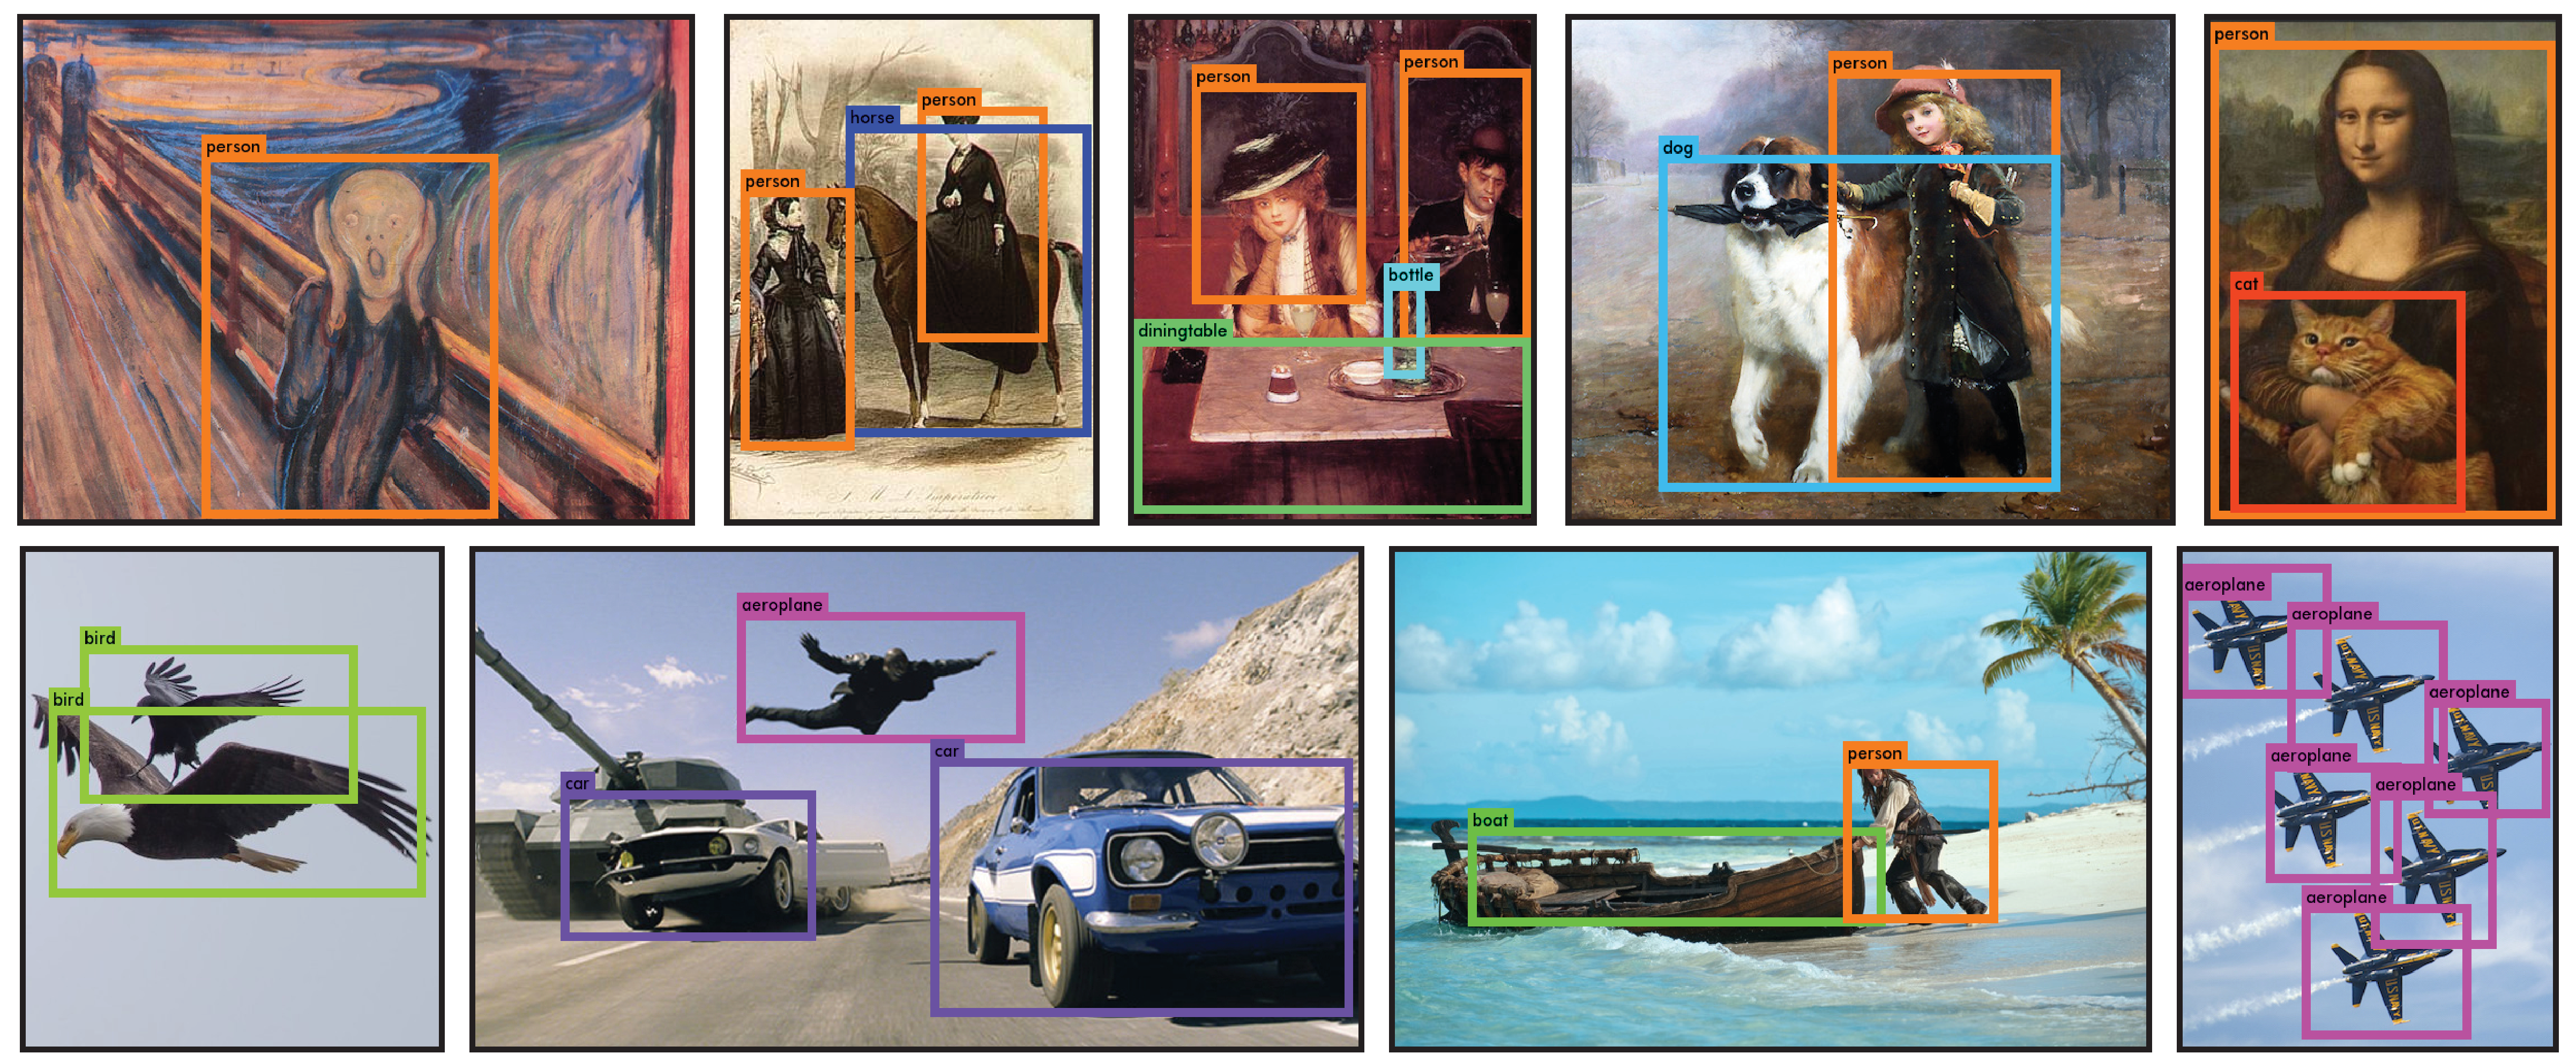
\includegraphics[width=0.9\textwidth]{./resources/images/redmon2016you_fig-6.pdf}
        \caption{Bounding Boxen in Bildern~\cite[Abb.~~6]{redmon2016you}}
        \label{fig:bounding_box}
    \end{figure}
\end{frame}

\begin{frame}{Intersection over Union (IoU)}
    \begin{columns}
        \begin{column}{0.6\textwidth}
            \begin{itemize}
                \item Wie gut ist eine Bounding Box?
                \item[]
                \item<2-> Intersection over Union (IoU)
                      \begin{itemize}
                          \item $IoU = \frac{A_{inter}}{A_{union}}$
                          \item $A_{inter}$: Fläche der Überlappung
                          \item $A_{union}$: Fläche der Vereinigung
                      \end{itemize}
                \item<2->[]
                \item<3-> IoU ist ein Maß für die Qualität der Bounding Box
                      \begin{itemize}
                          \item $IoU = 1$: Box passt perfekt
                          \item $IoU = 0$: Box passt gar nicht
                      \end{itemize}
            \end{itemize}
        \end{column}

        \begin{column}{0.4\textwidth}
            \begin{figure}
                \centering
                \only<2->{
                    \includegraphics[width=0.9\textwidth]{./resources/images/bishop2023deep_fig-10_20.pdf}
                    \caption{IoU~\cite[Abb.~~10.20]{bishop2023deep}}
                    \label{fig:iou_example}
                }
            \end{figure}
        \end{column}
    \end{columns}
\end{frame}

\begin{frame}{Precision und Recall}
    \begin{columns}
        \begin{column}{0.4\textwidth}
            \begin{itemize}
                \item $Precision = \frac{TP}{TP + FP}$
                \item $Recall = \frac{TP}{TP + FN}$
                \item[]

                      \only<2-3>{\item<2-3> $TP$: True Positives
                \item $FP$: False Positives
                \item $FN$: False Negatives
                      }

                \item<4->\textbf{Precision:}\\Wie viele der erkannten Objekte sind tatsächlich Objekte?\\$\rightarrow$ "`Treffsicherheit"'
                \item<5->\textbf{Recall:}\\Wie viele der tatsächlich vorhandenen Objekte wurden erkannt?\\$\rightarrow$ "`Erfassungsrate"'
            \end{itemize}
        \end{column}
        \begin{column}{0.6\textwidth}
            \begin{figure}
                \centering
                \only<2->{
                    \resizebox{0.9\textwidth}{!}{\begin{tikzpicture}[
        every node/.style={minimum size=1.2cm, anchor=center},
        every path/.style={draw},
        class/.style={font=\bfseries}
    ]

    % Matrix
    \matrix (confmat) [matrix of nodes, nodes in empty cells,
        nodes={draw, minimum width=1.8cm, minimum height=1.2cm, anchor=center},
        column sep=0.2cm, row sep=0.2cm,
        row 1/.style={nodes={draw=none, font=\bfseries}},
        column 1/.style={nodes={draw=none, font=\bfseries, rotate=90}},
    ] {
              & Hund & Katze & Maus \\
        Hund  & 45   & 2     & 1    \\
        Katze & 1    & 48    & 3    \\
        Maus  & 0    & 2     & 46   \\
    };

    % Labels
    \node[above=0.1cm of confmat-1-2] {Vorhergesagt (Predicted)};
    \node[rotate=90, left=1.0cm of confmat-2-1] {Tatsächlich (Actual)};

\end{tikzpicture}}
                    \caption{Confusion Matrix}
                    %\includegraphics[width=0.9\textwidth]{./resources/images/scikitlearn2025confusion_confusion_matrix.png}
                    %\caption{Confusion Matrix~\cite{scikitlearn2025confusion}}
                    \label{fig:confusion_matrix}
                }
            \end{figure}
        \end{column}
    \end{columns}
\end{frame}

\begin{frame}{Mean Average Precision (mAP)}
    \begin{columns}
        \begin{column}{0.6\textwidth}
            \begin{itemize}
                \item Wie gut ist ein Detektor?~\cite{everingham2010pascal,lin2014microsoft}
                \item[]
                \item<2-> Mean Average Precision (mAP)
                      \begin{itemize}
                          \item $mAP = \frac{1}{N} \sum_{i=1}^{N} AP_i$
                          \item $AP_i$: Average Precision für Klasse~$i$
                      \end{itemize}
                \item<2->[]
                \item<3-> Average Precision (AP)
                      \begin{itemize}
                          \item $AP_i = \int_0^1 P(r) dr$
                          \item $P(r)$: Precision bei Recall~$r$
                      \end{itemize}
            \end{itemize}
        \end{column}
        \begin{column}{0.4\textwidth}
            \begin{figure}
                \centering
                \only<3->{
                    \resizebox{0.9\textwidth}{!}{\begin{tikzpicture}
    \begin{axis}[
            xlabel={Recall},
            ylabel={Precision},
            axis lines=middle,
            xmin=0, xmax=1,
            ymin=0, ymax=1,
            grid=major,
            width=10cm,
            height=8cm,
            legend pos=south west,
        ]
        \addplot[thick, blue, domain=0:1, samples=100] { (1 - x^2)/(1 + x^2) };
        \addlegendentry{PR Curve}
        \addplot[fill=blue!20, domain=0:1, samples=100] { (1 - x^2)/(1 + x^2) } \closedcycle;
        \addplot[mark=*, mark size=3pt, red] coordinates {(0.5, 0.6)};
        \node at (axis cs:0.5,0.65) [font=\small, red] {Threshold};
    \end{axis}
\end{tikzpicture}}
                    \caption{PR-Kurve}
                    \label{fig:pr_curve}
                }
            \end{figure}
        \end{column}
    \end{columns}
\end{frame}

\begin{frame}{Regressionsausgabe}
    \begin{columns}
        \begin{column}{0.6\textwidth}
            \begin{itemize}
                \item Overfeat~\cite{sermanet2013overfeat} fügt den uns bereits bekannten CNNs eine zusätzliche Regressionsausgabe hinzu
                \item Diese vier Werte geben die Koordinaten der Bounding Box an (siehe Folie~\ref{frame:bounding_box})
            \end{itemize}
        \end{column}
        \begin{column}{0.4\textwidth}
            \begin{figure}
                \centering
                \only<2->{
                    \includegraphics[width=0.6\textwidth]{./resources/images/fleuret2022dlc_overfeat.png}
                    \caption{Zusätzliche Regressionsausgabe~\cite[Kapitel~8.3.2]{fleuret2022dlc}}
                    \label{fig:regression_output}
                }
            \end{figure}
        \end{column}
    \end{columns}
\end{frame}

\begin{frame}{Sliding Windows}\label{frame:sliding_windows}
    \begin{itemize}
        \item Einfaches Verfahren zur Objekterkennung
        \item Ein Fenster wird schrittweise über das Bild geschoben
        \item Für jeden "`Ausschnitt"' des Bildes wird ein CNN aufgerufen\\$\rightarrow$ enthält dieser Ausschnitt ein Objekt?
        \item[]
        \item<2-> \textbf{Nachteil:} Unglaublich rechenintensiv
    \end{itemize}
\end{frame}

\begin{frame}{Region Proposals}
    \begin{itemize}
        \item Algorithmen, die Regionen im Bild vorschlagen, die Objekte enthalten könnten
        \item Geschieht anhand von Bildmerkmalen\\(z.B. Farben, Kanten, Texturen)
        \item Reduktion der Anzahl der CNN Aufrufe im Vergleich zu Sliding Windows (siehe Folie~\ref{frame:sliding_windows})
    \end{itemize}
\end{frame}

\begin{frame}{Zweistufige Objektdetektoren}
    \only<1-2>{
        \begin{enumerate}
            \item Regionen werden vorgeschlagen
            \item Regionen werden klassifiziert und die Bounding Boxen werden berechnet
        \end{enumerate}
    }
    \begin{itemize}
        \item<2->[]
        \item<2-> Beispiele
              \begin{itemize}
                  \item R-CNN~\cite{girshick2014rich}
                        \only<3>{
                            \begin{itemize}
                                \item Selective Search~\cite{uijlings2013selective} generiert Regionen
                                \item Jede Region wird separat durch ein CNN verarbeitet
                                \item Features werden separat für Klassifikation (was ist es?) und Regression (wo ist es?) verwendet
                            \end{itemize}
                        }
                  \item Fast R-CNN~\cite{girshick2015fast}
                        \only<4>{
                            \begin{itemize}
                                \item Feature-Sharing: Das CNN verarbeitet das gesamte Bild nur einmal
                                \item End-to-End-Training: Zeitgleiches Training von Klassifikation und Regression
                            \end{itemize}
                        }
                  \item Faster R-CNN~\cite{ren2016faster}
                        \only<5>{
                            \begin{itemize}
                                \item Region Proposal Network (RPN): Regionsvorschläge direkt aus den CNN-Features
                                \item RPN teilt die CNN-Features mit dem Detektor
                            \end{itemize}
                        }
              \end{itemize}
    \end{itemize}
\end{frame}

\begin{frame}{Einstufige Objektdetektoren}
    \only<1-2>{
        \begin{itemize}
            \item Alles in einem Schritt
            \item Gesamtes Bild als Eingabe (keine Regionen)
            \item Direkte Vorhersage der Bounding Boxen \textbf{und} Klassen
        \end{itemize}
    }
    \begin{itemize}
        \item<2->[]
        \item<2-> Beispiele
              \begin{itemize}
                  \item YOLO~\cite{redmon2016you}
                        \only<3>{
                            \begin{itemize}
                                \item Bild wird in ein $S \times S$ Gitter unterteilt
                                \item Für jede Zelle werden Bounding Boxen ($B$) und Klassenwahrscheinlichkeiten ($C$) vorhergesagt
                            \end{itemize}
                        }
                  \item SSD~\cite{liu2016ssd}
                        \only<4>{
                            \begin{itemize}
                                \item Fügt zusätzliche Faltungen (Feature Maps) hinzu
                                \item Ermöglicht einfachere Vorhersage von Objekten mit unterschiedlichen Größen
                                \item Vorhersage der Bounding Boxen und Klassen dann auf jeder Feature Map
                            \end{itemize}
                        }
              \end{itemize}
    \end{itemize}
\end{frame}

\begin{frame}{YOLO}
    \begin{figure}
        \centering
        \includegraphics[width=0.9\textwidth]{./resources/images/redmon2016you_fig-2.pdf}
        \caption{YOLO Modell, $7 \times 7$ Gitter~\cite[Abb.~2]{redmon2016you}}
        \label{fig:yolo_model}
    \end{figure}
\end{frame}

\begin{frame}{YOLO}
    \begin{figure}
        \centering
        \includegraphics[width=0.9\textwidth]{./resources/images/redmon2016you_fig-3.pdf}
        \caption{YOLO Architektur~\cite[Abb.~3]{redmon2016you}}
        \label{fig:yolo_architecture}
    \end{figure}
    \only<2->{
        \begin{itemize}
            \item Alle Komponenten sind uns bereits bekannt
                  \begin{itemize}
                      \item 24 Convolutional Layer
                      \item 2 Fully Connected Layer
                      \item Maxpooling Layers
                      \item (Leaky) ReLU Aktivierungsfunktionen
                      \item Output: $S \times S \times (B \times 5 + C)$, hier mit $S=7$, $B=2$, $C=20$
                  \end{itemize}
        \end{itemize}
    }
\end{frame}

\begin{frame}{YOLO}
    \begin{itemize}
        \item Stetige Weiterentwicklung
        \item YOLOv1 (2016) -- YOLOv11 (2024)
        \item[]
        \item<2-> Integration in eigene Projekte wird immer einfacher~\cite{ultralytics2025yolo}
              \begin{itemize}
                  \item \texttt{pip install ultralytics}
                  \item \texttt{from ultralytics import YOLO}
                  \item \texttt{model = YOLO("yolo11n.pt")}
                  \item \texttt{results = model.predict(source="video.mp4")}
                  \item \texttt{results[0].plot()}
              \end{itemize}
    \end{itemize}
\end{frame}

\begin{frame}{Zusammenfassung}
    \begin{itemize}
        \item<1-> Objekterkennung als wichtiges Anwendungsgebiet von CNNs
        \item<2-> Unterscheidung zwischen
              \begin{itemize}
                  \item Zweistufige Detektoren (z.B. R-CNN, Fast R-CNN, Faster R-CNN)
                  \item Einstufige Detektoren (z.B. \textbf{YOLO}, SSD)
              \end{itemize}
        \item<3-> Grundsätzlich sind zweistufige Detektoren genauer und einstufige Detektoren schneller
        \item<4-> YOLO immer mehr Beliebtheit, da Echtzeit-Objekterkennung unglaublich spannendes Anwendungsgebiet
    \end{itemize}
\end{frame}

\begin{frame}{Ausblick}
    \begin{itemize}
        \item Bildsegmentierung
        \item Transformer-basierte Detektoren (z.B. DETR~\cite{carion2020end})
    \end{itemize}
\end{frame}

\begin{frame}[allowframebreaks, noframenumbering, plain]{Quellen}
    \sloppy
    \printbibliography
\end{frame}

\end{document}